%!TEX root = ../../../_main.tex
\section{Twisted involutions in Coxeter groups}
\label{sec:twisted-involutions}

In this section we focus on a certain subset of elements in Coxeter groups, the so called twisted involutions. From now on (and in the next sections) we fix some symbols to have always the same meaning (some definitions follow later):

\vspace*{1em}

\begin{tabular}{rl}
	$(W,S)$			& A Coxeter system with generators $S$ and elements $W$.\\
	$s$				& A generator in $S$.\\
	$u,v,w$			& A element in the Coxeter group $W$.\\
	$m_{ij}$		& The order of the element $(s_i s_j)$ with $s_i$ the $i$-th generator of $W$.\\
	$\theta$		& A Coxeter system automorphism of $(W,S)$ with $\theta^2 = \id$.\\
	$\ti{\theta}$	& The set of $\theta$-twisted involutions of $W$.\\
	$\ul S$			& A set of symbols, $\ul S = \{ \ul s : s \in S \}$.\\
\end{tabular}

\subsection{Introduction to twisted involutions}
\label{sec:twisted-involutions-introduction}

\begin{defi}
	Let $(W,S)$ be a Coxeter system. An automorphism $\theta : W \to W$ with $\theta(S) = S$ is called a \defword{Coxeter system automorphism} of $(W,S)$.
\end{defi}

\begin{defi}
	Let $(W,S)$ be a Coxeter system and $\theta : W \to W$ a Coxeter system automorphism. Then each $w \in W$ with $\theta(w) = w^{-1}$ is called a \defword{twisted involution}. The set of all twisted involutions in $W$ regarding $\theta$ is denoted with $\ti{\theta}(W)$. Often we will just omit the Coxeter group and write $\ti{\theta}$, when it is clear from the context which $W$ is meant.
\end{defi}

Lets take a quick look at some examples. First of all the trivial one.

\begin{exam}
	Let $(W,S)$ be a Coxeter system and $\theta = \id_W$. Then $\theta$ is an Coxeter system automorphism and $\ti{\theta} = \{ w \in W : w = w^{-1} \}$.
\end{exam}

The next example is more helpfull, since it reveals a way to think of $\ti{\theta}$ as a generalization of ordinary Coxeter groups.

\begin{exam}
	Let $(W,S)$ be a Coxeter system and $\theta$ be the automorphis (not Coxeter system automorphism)
	$$ \theta : W \times W \to W \times W : (u,w) \mapsto (w,u). $$
	Then the set of twisted involutions is $\ti{\theta} = \{ (w,w^{-1}) \in W \times W : w \in W \}$. This yields a canonical bijection between $\ti{\theta}$ and $W$.
\end{exam}
\subsection{Twisted weak ordering}
\label{sec:twisted-involutions-twisted-weak-ordering}

In this section we will introduce the twisted weak ordering $Wk(\theta)$ on Coxeter groups. 

%TODO
TODO
%!TEX root = ../../../_main.tex
\subsection{Residuums}
\label{sec:twisted-involutions-residuums}

\begin{defi}
	\typedlabel{defi:residuum}
	Let $w \in W$ and $I \subseteq S$ be a subset of generators. Then we define
	$$ wC_I := \{ w \ul s_1 \ldots \ul s_k : k \in \nn_0, s_i \in S \} $$
	as the \defword{$I$-residuum} of $w$ or just \defword{residuum}. To emphasize the size of $I$, say $|I| = n$, we also speak of a \defword{rank-$n$-residuum}.
\end{defi}

\begin{exam}
	Let $w \in W$. Then $wC_\emptyset = \{ w \}$ and $wC_S = \ti{\theta}$.
\end{exam}

\begin{lemm}
	\typedlabel{lemm:all-elements-of-one-residuum-yield-the-same-residuum}
	Let $w \in W$ and $I \subset S$. If $v \in wC_I$, then $vC_I = wC_I$.

	\begin{proof}
		Suppose $v \in wC_I$. Then $v = w \ul s_1 \ldots \ul s_n$ for some $s_i \in I$. Suppose $u = w \ul t_1 \ldots \ul t_m \in wC_I$ is any other element in $wC_I$ with $t_i \in I$. Then
		$$ u = w \ul t_1 \ldots \ul t_m = (v \ul s_n \ldots \ul s_1) \ul t_1 \ldots \ul t_m $$
		and so $u \in vC_I$. This yields $wC_I \subset vC_I$. Since $w \in vC_I$ we can swap $v$ and $w$ to get the other inclusion.
	\end{proof}
\end{lemm}

\begin{coro}
	Let $v, w \in W$ and $I \subset S$. Then either $vC_I \cap wC_I = \emptyset$ or $vC_I = wC_I$.

	\begin{proof}
		Immediately follows from \ref{lemm:all-elements-of-one-residuum-yield-the-same-residuum}.
	\end{proof}
\end{coro}

\begin{prop}
	\typedlabel{prop:residuums-have-unique-wk-theta-minimal-element}
	Let $w \in \ti{\theta}$, $I \subseteq S$ be a set of generators. Then there exists a unique element $w_0 \in wC_I$ with $w_0 \preceq w_0 \ul s$ for all $s \in I$.

	\begin{proof}
		Suppose there is no such element. Then for each $w \in wC_I$ we can find a $s \in I$ with $w' = w \ul s \preceq w$ and $e' \in wC_I$. By repetition \ref{prop:deletion-property-for-twisted-expressions} says, that $e \in wC_I$, but $e$ has the property, which we assumed, that no element in $wC_I$ has. Hence there must be at least one such element. Now suppose there are two distinct elements $u,v$ with the desired property. Note that this means, that $u$ and $w$ have no reduced twisted expression ending with some $\ul s \in I$. Let $v$ have a reduced twisted expression $v = \ul s_1 \ldots \ul s_k$. Since $u$ and $v$ are both in $wC_I$ there must be a twisted $v$-expression for $u$
		$$ u = v \ul s_{k+1} \ldots \ul s_{k+l} = \ul s_1 \ldots \ul s_{k+l} $$
		with $s_n \in I$ for $k+1 \leq n \leq k+l$. This twisted expression cannot be reduced, since it ends with $\ul s_{k+l} \in I$. Then \ref{prop:deletion-property-for-twisted-expressions} yields that this twisted expression contains a reduced twisted subexpression for $u$. It cannot end with $\ul s_n$ for $k+1 \leq n \leq k+l$. Hence it is a twisted subexpression of $\ul s_1 \ldots \ul s_k = v$, too. So $u \leq v$ by \ref{theo:bruhat-subexpression-characterization}. Because of symmetry it is also $v \leq u$ and so $u = v$, contradicting to our assumption $u \neq v$.
	\end{proof}
\end{prop}

\begin{coro}
	\typedlabel{coro:residuums-have-unique-minimal-element}
	Let $w \in \ti{\theta}$, $I \subseteq S$ be a set of generators and let $\rho_{min} := \{ \rho(v) : v \in wC_I \}$ be the minimal twisted length within the residuum $wC_I$. Then there is a unique element $w_{min} \in wC_I$ with $\rho(w_{min}) = \rho_{min}$. We denote this element with $\min(w,I)$.

	\begin{proof}
		The minimal rank $\rho_{min}$ exists, since $\rho : \ti{\theta} \to \nn_0$, $\nn_0$ is well-ordered and $wC_I \neq \emptyset$. Suppose we have an element $w_{min}$ with $\rho(w_{min}) = \rho_{min}$. This means, that in particular all $w_{min} \ul s$ with $s \in I$ must be of larger twisted length, i.e. $w_{min} < w_{min} \ul s$ for all $s \in I$. With \ref{prop:residuums-have-unique-wk-theta-minimal-element} this element must be unique.
	\end{proof}
\end{coro}

We proceed with some properties of rank-2-residuums. Our interest in these residuums steems from the fact, that their properties are needed later in Section \ref{sec:twisted-involutions-algorithms} to construct an effective algorithm for calculating the twisted weak ordering, i.e. calculating the Hasse diagram of $Wk(\theta)$ for arbitrary Coxeter systems $(W,S)$ and Coxeter system automorphisms $\theta$.

\begin{defi}
	Let $s,t \in S$ be two distinct generators. We define:
	$$[\ul s \ul t]^n :=
	\begin{cases}
	(\ul s \ul t)^{\frac{n}{2}} & n \textrm{ even}, \\
	(\ul s \ul t)^{\frac{n-1}{2}} \ul s & n \textrm{ odd}. 
	\end{cases}$$
\end{defi}

This definition lets us rewrite rank-2-residuums. Suppose we have an element $w \in \ti{\theta}$ and two distinct generators $s,t \in S$. Thanks to \ref{lemm:all-elements-of-one-residuum-yield-the-same-residuum} and \ref{coro:residuums-have-unique-minimal-element} we can assume, that $w = min(w,\{s,t\})$. Then
$$ wC_{\{s,t\}} = \{ w \} \ \cup \ \{ w [\ul s \ul t]^n : n \in \nn \} \ \cup \ \{ w [\ul t \ul s]^n : n \in \nn \}. $$
This encourages the following definition.

\begin{defi}
	Let $w \in \ti{\theta}$ and let $s,t \in S$ be two distinct generators. Suppose $w = min(w,\{s,t\})$. Then we call $\{ w [\ul s \ul t]^n : n \in \nn \}$ the \defword{$s$-branch} and $\{ w [\ul t \ul s]^n : n \in \nn \}$ the \defword{$t$-branch} of $wC_{\{s,t\}}$.
\end{defi}

One question arises immediately: Are the $s$- and the $t$-branch disjoint? With the following propositions, corollaries and lemmas we will get a much better idea of the structure of rank-2-residuums and answer this question.

\begin{prop}
	\typedlabel{prop:rank-2-residuums-are-convex}
	Let $w \in W$ and let $s,t \in S$ two distinct generators. Without loss of generality suppose $w = \min(w, \{s,t\})$. If there is a $v \in wC_{\{s,t\}}$ with $v \ul s \prec v$ and $v \ul t \prec v$, then it is the unique element with this property forcing $wC_{\{s,t\}}$ to consist of two geodesics from $w$ to $v$ intersecting only in this two elements. Else the $s$- and $t$-branch are disjoint, strictly ascending in twisted length and of infinite size.

	\begin{proof}
		Suppose there is a $v$ in the $s$-branch with $v \ul s \prec v$ and $v \ul t \prec v$, say $v = w[\ul s \ul t]^n$. Then $w[\ul s \ul t]^{m+1} \prec w[\ul s \ul t]^m$ for $n \leq m \leq 2m - 1$ and $w[\ul s \ul t]^{2n} = w$. This is because assuming the opposite would yield an element $u \neq w$ with $u \prec u \ul s$ and $u \prec u \ul t$ contradicting to the uniqueness from \ref{prop:residuums-have-unique-wk-theta-minimal-element}. If no such $v$ exists, then the $s$- and $t$-branch must be disjoint, strictly ascending in twisted length and so of infinite size.
	\end{proof}
\end{prop}

\begin{prop}
	\typedlabel{prop:onesided-operations-only-at-top-or-bottom-end-of-twocycle}
	Let $w \in S$ and $s,t \in S$ two distinct generators. If $s$ operates onesided on $w$ and $w \ul s \prec w$, then either $w \ul{st} \prec w \ul{s}$ or $w \ul{t} \succ w$.

	\begin{proof}
		We have $\theta(s)ws = w$ and $s \in D_R(w)$. If $t \notin D_R(w)$, then we are done. So suppose $t \in D_R(w)$. This means $w \ul s \leq w$ and $w \ul t \leq w$ and \cite[Lemma 3.9]{hultman:comb-twisted-invo} yields $w \ul {st} < w$ and $w \ul {ts} < w$. If $t \in D_R(w \ul s)$, then we are done. So suppose $t \notin D_R(w \ul s)$. Then $t \in D_R(w \ul {st})$. Together with $w \ul {st} \leq w$ \cite[Lemma 3.9(2)]{hultman:comb-twisted-invo} says $(w \ul {st}) \ul t \leq w \ul t$. Finally we get
		$$ ws = w \ul s = (w \ul {st}) \ul t \leq w \ul t = wt.$$
		Since $w \ul s$ and $w \ul t$ are of same twisted length they have to be equal and therefore $s = t$ which contradicts to our assumption of two distinct generators $s$ and $t$. We now have $w \ul s \ul t < w \ul s$ or $w \ul t > w$ (in $\Br(\ti{\theta})$). Both cases can be transfered to the twisted weak ordering. If $w \ul s \ul t < w \ul s$, then $\rho(w \ul s \ul t) = \rho(w \ul s) - 1$ and $w \ul s \ul t \ul t = w \ul s$, yielding $w \ul s \ul t \prec w \ul s$. If $w \ul t > w$ then $\rho(w \ul t) = \rho(w) + 1$, yielding $w \ul t \succ w$.
	\end{proof}
\end{prop}

\begin{coro}
	\typedlabel{coro:onesided-operations-only-at-top-or-bottom-end-of-twocycle}
	Let $w \in S$ and let $s,t \in S$ be two distinct generators. If $w$ is neither the unique element in $wC_{\{s,t\}}$ of smallest twisted length,i.e. $\min(w,\{s,t\})$, nor the unique (but not necessarily existing) element of largest twisted length, then both $s$ and $t$ act twosided on $w$.

	\begin{proof}
		Follows immediately from \ref{prop:onesided-operations-only-at-top-or-bottom-end-of-twocycle}.
	\end{proof}
\end{coro}

\begin{lemm}
	\typedlabel{lemm:max-twisted-circle-height}
	Let $w \in S$, $s,t \in S$ two distinct generators and $m = \ord(st) < \infty$. Then $|wC_{\{s,t\}}| \leq 2m$.

	\begin{proof}
		\todo
	\end{proof}
\end{lemm}

\begin{exam}
	In Figure \ref{fig:a4_s1s3-and-a4_s2s4} we see two Hasse diagrams of $Wk(A_4, \id)$. The first only contains edges with label $s_1,s_3$ and the second only edges with label $s_2,s_4$.
	\begin{figure}[ht]
		\centering
		%!TEX root = ../../_main.tex
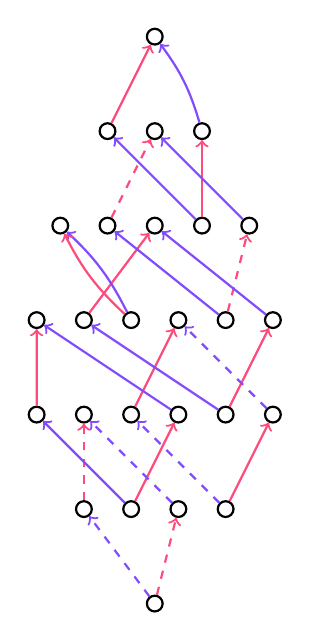
\begin{tikzpicture}[scale=0.8,bend angle=10]
\newcommand{\xspace}{1}
\newcommand{\yspace}{1}
\tikzstyle{vertex}=[draw,thick,circle,minimum size=2mm,inner sep=0pt]
\tikzstyle{edge}=[thick,->]
\tikzstyle{onesided}=[edge,dashed]
\tikzstyle{bothsided}=[edge]
\tikzstyle{unhighlighted}=[]
\tikzstyle{highlighted}=[]
\definecolor{s1color}{RGB}{130,76,253}
\definecolor{s2color}{RGB}{76,253,78}
\definecolor{s3color}{RGB}{253,76,124}
\definecolor{s4color}{RGB}{76,176,253}
\tikzstyle{s1}=[s1color]
\tikzstyle{s2}=[s2color]
\tikzstyle{s3}=[s3color]
\tikzstyle{s4}=[s4color]
\node[vertex,unhighlighted] (0) at (\xspace*0,\yspace*0) {};
\node[vertex,unhighlighted] (1) at (\xspace*-1.125,\yspace*1.5) {};
\node[vertex,unhighlighted] (2) at (\xspace*-0.375,\yspace*1.5) {};
\node[vertex,unhighlighted] (3) at (\xspace*0.375,\yspace*1.5) {};
\node[vertex,unhighlighted] (4) at (\xspace*1.125,\yspace*1.5) {};
\node[vertex,unhighlighted] (5) at (\xspace*-1.875,\yspace*3) {};
\node[vertex,unhighlighted] (6) at (\xspace*-1.125,\yspace*3) {};
\node[vertex,unhighlighted] (7) at (\xspace*-0.375,\yspace*3) {};
\node[vertex,unhighlighted] (8) at (\xspace*0.375,\yspace*3) {};
\node[vertex,unhighlighted] (9) at (\xspace*1.125,\yspace*3) {};
\node[vertex,unhighlighted] (10) at (\xspace*1.875,\yspace*3) {};
\node[vertex,unhighlighted] (11) at (\xspace*-1.875,\yspace*4.5) {};
\node[vertex,unhighlighted] (12) at (\xspace*-1.125,\yspace*4.5) {};
\node[vertex,unhighlighted] (13) at (\xspace*-0.375,\yspace*4.5) {};
\node[vertex,unhighlighted] (14) at (\xspace*0.375,\yspace*4.5) {};
\node[vertex,unhighlighted] (15) at (\xspace*1.125,\yspace*4.5) {};
\node[vertex,unhighlighted] (16) at (\xspace*1.875,\yspace*4.5) {};
\node[vertex,unhighlighted] (17) at (\xspace*-1.5,\yspace*6) {};
\node[vertex,unhighlighted] (18) at (\xspace*-0.75,\yspace*6) {};
\node[vertex,unhighlighted] (19) at (\xspace*0,\yspace*6) {};
\node[vertex,unhighlighted] (20) at (\xspace*0.75,\yspace*6) {};
\node[vertex,unhighlighted] (21) at (\xspace*1.5,\yspace*6) {};
\node[vertex,unhighlighted] (22) at (\xspace*-0.75,\yspace*7.5) {};
\node[vertex,unhighlighted] (23) at (\xspace*0,\yspace*7.5) {};
\node[vertex,unhighlighted] (24) at (\xspace*0.75,\yspace*7.5) {};
\node[vertex,unhighlighted] (25) at (\xspace*0,\yspace*9) {};
\draw[s1,onesided,unhighlighted] (0) edge (1);
\draw[s3,onesided,unhighlighted] (0) edge (3);
\draw[s3,onesided,unhighlighted] (1) edge (6);
\draw[s1,bothsided,unhighlighted] (2) edge (5);
\draw[s3,bothsided,unhighlighted] (2) edge (8);
\draw[s1,onesided,unhighlighted] (3) edge (6);
\draw[s1,onesided,unhighlighted] (4) edge (7);
\draw[s3,bothsided,unhighlighted] (4) edge (10);
\draw[s3,bothsided,unhighlighted] (5) edge (11);
\draw[s3,bothsided,unhighlighted] (7) edge (14);
\draw[s1,bothsided,unhighlighted] (8) edge (11);
\draw[s1,bothsided,unhighlighted] (9) edge (12);
\draw[s3,bothsided,unhighlighted] (9) edge (16);
\draw[s1,onesided,unhighlighted] (10) edge (14);
\draw[s3,bothsided,unhighlighted] (12) edge (19);
\draw[s1,bothsided,unhighlighted,bend right] (13) edge (17);
\draw[s3,bothsided,unhighlighted,bend left] (13) edge (17);
\draw[s1,bothsided,unhighlighted] (15) edge (18);
\draw[s3,onesided,unhighlighted] (15) edge (21);
\draw[s1,bothsided,unhighlighted] (16) edge (19);
\draw[s3,onesided,unhighlighted] (18) edge (23);
\draw[s1,bothsided,unhighlighted] (20) edge (22);
\draw[s3,bothsided,unhighlighted] (20) edge (24);
\draw[s1,bothsided,unhighlighted] (21) edge (23);
\draw[s3,bothsided,unhighlighted] (22) edge (25);
\draw[s1,bothsided,unhighlighted,bend right] (24) edge (25);
\end{tikzpicture}
		\quad \quad \quad
		\input{resources/tikz/a4_s2s4}
		\caption{Hasse diagrams of $Wk(A_4, \id)$ with only $s_1,s_3$ edges on the left and only $s_2,s_4$ edges on the right side}
		\label{fig:a4_s1s3-and-a4_s2s4}
	\end{figure}
\end{exam}
\subsection{Twisted weak ordering algorithms}
\label{sec:twisted-involutions-algorithms}